\documentclass{article}
\usepackage[utf8]{inputenc}
\usepackage[document]{ragged2e}
\usepackage{algpseudocode}
\usepackage[]{algorithmicx}
\usepackage{amsmath}
\usepackage{amsthm}
\usepackage{amssymb}
\usepackage[]{listings}
\usepackage{graphicx}
\usepackage{hyperref}
\usepackage{flafter}
\usepackage{subfig}
\usepackage{dsfont}
\graphicspath{ {images/} }

\begin{document}

\begin{titlepage}
	\centering
	%
\includegraphics[width=0.15\textwidth]{IIIT-B_logo.jpg}\par\vspace{1cm}
	{\scshape\LARGE International Institute of Information Technology, Bangalore \par}
	\vspace{1cm}
	{\scshape\Large Project Strategy Document\par}
	{\Large  DS 707 Data Analytics\par}
	\vspace{1.5cm}
	{\huge\bfseries Exploratory Analytics and Classification \par}
	\vspace{2cm}
	{\Large\itshape Akanksha Dwivedi - MT2016006\par}
	{\Large\itshape Hitesha Mukherjee - MS2016007\par}
	{\Large\itshape Nayna Jain - MS2017003\par}
	{\Large\itshape Tarini Chandrashekhar - MT2016144\par}
	\vfill
	Instructors : \par
	Prof. Ramanathan Chandrashekhar
	\par
	Prof. Uttam Kumar

	\vfill
% Bottom of the page
	{\large \today\par}
\end{titlepage}

\newpage

\tableofcontents

\newpage
\justify

\

\section{Data Exploration}

\subsection {Introduction}
Multivariate time series (MTS) data sets are common in many multimedia, medical, process industry and financial applications such as gesture recognition, video sequence matching, EEG/ECG data analysis or prediction of abnormal situation or trend of stock price. MTS data sets are high dimensional as they consist of a series of observations of many variables (multidimendsional variable) at a time.[1]
For analysis of MTS data in order to extract knowledge, a compact representation is needed. For feature subset selection for MTS data sets, popular techniques for machine learning or pattern recognition problems are modified. [1] \newline

Any data mining or pattern recognition task such as
knowledge/rule extraction, clustering or classification of data is preceeded by data preprocessing.[1] Preprocessing of data is the process in which redundant or irrelevant information from the data is removed while the most discriminatory information is retained to represent the data in a compact manner. This preprocessing stage is often known as feature extraction or feature subset selection.[1] The next step for classification or clustering is to design a similarity measure for identifying similar time series to make clusters or classes or to extract rules.[1]

\subsubsection {Time Series Classification}
Our data is based on mining Bitcoin and Etherium crypto currencies. Basically our data is a Historical Timeseries data.It has wide variety of features.
Time series classification is to build a classification model based on labelled time series and then use the model to predict the label of unlabelled time series.[2] The way for time series classification with R is to extract and build features from time series data first, and then apply existing classification techniques, such as SVM, k-NN, neural networks, regression and decision trees, to the feature set.[2]

\subsection{Selecting Appropriate Classification
Technique }

\subsubsection {Supervised versus Unsupervised learning} This is one of the most fundamental distinctions between learning methods.[3] Supervised learning involves developing descriptions froma pre-classified set of training examples, where the classifications are assigned by an expert in the problem domain.[3] The aim is to produce descriptions that will accurately classify unseen test examples. In unsupervised learning, no prior classification is provided, and it is up to the learning scheme itself to generate one based on its analysis of the training data.[3] \newline

We have used Supervised Learning Model for classification of our dataset.In machine learning, support vector machines (SVMs, also support vector networks) are supervised learning models with associated learning algorithms that analyze data used for classification and regression analysis. [3]


\subsection {Build Classification Model Parameter Setting}

We manually select 16 features from the bit\textunderscore dataset\textunderscore cleaned\textunderscore filtered.csv,namely:
\begin{itemize}
\item Trade Volume
\item Total Bitcoins
\item Average Block Size
\item n\textunderscore Orphaned blocks
\item n\textunderscore Transactions per block
\item Median Confirmation time
\item Hash Rate
\item Transaction Fees
\item n\textunderscore Unique\textunderscore Addresses
\item n\textunderscore Transactions    
\item Cost per transaction Difficulty
\item Estimated Transaction Volume Hash Rate
\item Market Capitalization
\item Miners Revenue
\item Number of unique addresses Total Bitcoins
\item Trade Volume Transaction to trade ratio
\end{itemize}

We have chosen the names and descriptions of the 16 features that relate to the Bitcoin network. We leveraged these features in developing a binary and a ternary classification algorithm to predict the sign change in Bitcoin price based on daily data points. The binary classification algorithm predicts positive and no change as 1 and negative price change as -1. The ternary classification algorithm predicts positive price change as 1, negative price change as -1, and no change as 0. We used the results of the following classification algorithms and compared their results.\newline

We have considered the Bitcoin Dataset which has 24 features or attributes in it. We have extracted 16 important features and build a subset of the data as per the binary and ternary classification mentioned above. We have further classified our data into training and test data. 75 percentage of data is classified as Training and the rest as testing data. We have used the different algorithms mentioned below to build the model based on the training data and predicted the Market\textunderscore Price\textunderscore Label based on Model built and Test Data.

We tried to do predictive analysis using Linear Regression on Bitcoin Price Dataset. The data is divided into training and test data. The training data is 75\% sampled
from bitcoin\_price dataset and rest is 25\%. We have prepared a simple model of estimating Open Prices based on Market Capitalization. The independent variable is Market Capitalization and estimation is done for Open Price.

\subsubsection {Support Vector Machine for Classification}

“Support Vector Machine” (SVM) is a supervised machine learning algorithm which can be used for both classification or regression challenges.[4] In this algorithm, we plot each data item as a point in n-dimensional space (where n is number of features you have) with the value of each feature being the value of a particular coordinate. Then, we perform classification on them.[4] \newline

Some important parameters having higher impact on model performance, “kernel”, “gamma” and “C”
kernel: Here, we have various options available with kernel like, “linear”, “rbf”,”poly” and others (default value is “rbf”).  Here “rbf” and “poly” are useful for non-linear hyper-plane, we have used polynomial. Higher the value of gamma, will try to exact fit the as per training data set i.e. generalization error and cause over-fitting problem. C: Penalty parameter C of the error term. It also controls the trade off between smooth decision boundary and classifying the training points correctly.[4] \newline

Pros:
\begin{itemize}
\item It works really well with clear margin of separation.
\item It is effective in high dimensional spaces.
\item It is effective in cases where number of dimensions is greater than the number of samples.
\item It uses a subset of training points in the decision function (called support vectors), so it is also memory efficient.
\end{itemize}
Cons:
\begin{itemize}
\item It doesn’t perform well,when we have large data set because the required training time is higher
It also doesn’t perform very well, when the data set has more noise i.e. target classes are overlapping
SVM doesn’t directly provide probability estimates, these are calculated using an expensive five-fold cross-validation. 
\end{itemize}
\subsubsection {Random Forest for Classification}


\subsubsection {Naive Bayes Algorithm}

It is a classification technique based on Bayes’ Theorem with an assumption of independence among predictors. In simple terms, a Naive Bayes classifier assumes that the presence of a particular feature in a class is unrelated to the presence of any other feature.Naive Bayes model is easy to build and particularly useful for very large data sets.[4] \newline

Pros:
\begin{itemize}
\item It is easy and fast to predict class of test data set. It also perform well in multi class prediction,When assumption of independence holds, a Naive Bayes classifier performs better compare to other models like logistic regression and you need less training data. [4] \newline 
\end{itemize}

Cons:
\begin{itemize}
\item It performs well in case of categorical input variables compared to numerical variable.[4] \newline

\item If categorical variable has a category (in test data set), which was not observed in training data set, then model will assign a 0 (zero) probability and will be unable to make a prediction.[4] This is often known as “Zero Frequency”. To solve this, we can use the smoothing technique. One of the simplest smoothing techniques is called Laplace estimation.
On the other side naive Bayes is also known as a bad estimator, so the probability outputs are not to be taken too seriously.[4] \newline

\item Another limitation of Naive Bayes is the assumption of independent predictors. In real life, it is almost impossible that we get a set of predictors which are completely independent.[4]

\end{itemize}

\subsubsection{Linear Regression}

Linear Regression is used for predictive analysis. In this case, there is a response variable whose outcome has to be predicted based on the input variables which are also called as dependent variables. Linear Regression is used with continuous type of data. 

Pros:
\begin{itemize}
	\item Useful based on relationships between two quantitative continuous variables.
\end{itemize}

Cons:
\begin{itemize}
	\item Sensitive to outliers.
	\item Limitations in the shapes that linear models can assume over long ranges.
\end{itemize}

\subsection {Comparing the Different Classification Models Built}

\subsubsection{Linear Regression Model}

The mean square error which we got was  0.2127196982.
Figure 1 below shows the predicted vs actual value.

\begin{figure}
	\centering
	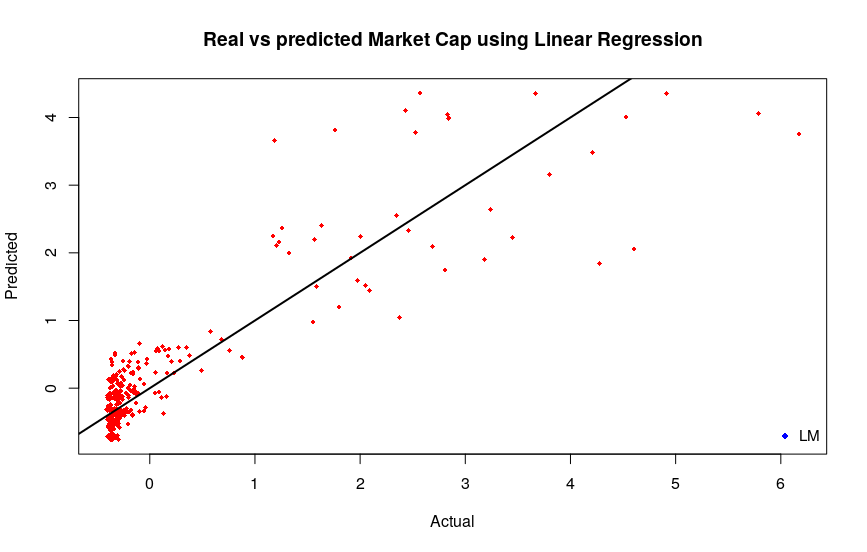
\includegraphics[width=\linewidth]{charts/bitcoin_market_cap_using_LR}
	\caption{Bitcoin Market Cap Prediction based on Open Price}
	\label{fig:Bitcoin Market Cap Prediction}
\end{figure}


\subsection {Visualizing Using Tableau}



\begin{thebibliography}{References}
\bibitem{1} Feature Selection and Classification Techniques for Multivariate Time Series
Basabi Chakraborty ;Faculty of Software and Information Science, Iwate Prefectural University - 152-52 Sugo, Takizawa-mura, Iwate, 020-0193, Japan E-mail: basabi@soft.iwate-pu.ac.jp.\newline

\bibitem{2} Article at the website http://www.rdatamining.com/examples/time-series-clustering-classification.\newline

\bibitem{3} The Application of Machine Learning Techniques to Time-Series Data - Author Scott Mitchell; Master of Computing and Mathematical Sciences at the University of Waikato. \newline

\bibitem{4} Article by Sunil Ray at Analytics Vidhya Website

\bibitem{5} Predicting the direction of stock market prices using random forest. Luckyson Khaidem Snehanshu Saha Sudeepa Roy Dey. khaidem90@gmail.com snehanshusaha@pes.edu sudeepar@pes.edu

\bibitem{5} Forecasting of Indian Stock Market Index Using Artificial Neural Network Manna Majumder1 , MD Anwar Hussian2

\bibitem{6} Stock Price Prediction Using Regression Analysis Dr. P. K. Sahoo, Mr. Krishna charlapally

\end{thebibliography}
\end{document}